\documentclass[a4paper]{article}
\usepackage{graphicx}
\usepackage{fullpage}
\usepackage{graphicx} % for pdf, bitmapped graphics files
\usepackage{amsmath} % assumes amsmath package installed
\usepackage{amssymb}  % assumes amsmath package installed\ref
\usepackage{psfrag}
\usepackage{algorithmic}
\usepackage{algorithm}
\usepackage{color}
\usepackage{xcolor}
\usepackage{listings}
\begin{document}

\lstset{
language=C++,
captionpos=b,
tabsize=2,
keywordstyle=\color{blue},
commentstyle=\color{green},
stringstyle=\color{red},
breaklines=true,
showstringspaces=false,
frame=shadowbox,
rulesepcolor=\color{gray},
basicstyle=\footnotesize%
}


\newcommand{\gopt}{g\ensuremath{^2}o}
\newcommand{\defeq}{\stackrel{\text{def.}}{=}}
\newcommand{\gcomment}[1]{\textcolor{red}{\textbf{Giorgio:}~\emph{#1}}}
\newcommand{\rcomment}[1]{\textcolor{red}{\textbf{Rainer:}~\emph{#1}}}

\def\secref#1{Section~\ref{#1}}
\def\figref#1{Figure~\ref{#1}}
\def\tabref#1{Table~\ref{#1}}
\def\eqref#1{Eq.~\ref{#1}}

\newcommand{\Dom}{\mathtt{Dom}}
\newcommand{\bZero}{\mathbf{0}}
\newcommand{\bb}{\mathbf{b}}
\newcommand{\bc}{\mathbf{c}}
\newcommand{\bh}{\mathbf{h}}
\newcommand{\bH}{\mathbf{H}}
\newcommand{\bA}{\mathbf{A}}
\newcommand{\bM}{\mathbf{M}}
\newcommand{\bF}{\mathbf{F}}
\newcommand{\bG}{\mathbf{G}}
\newcommand{\bI}{\mathbf{I}}
\newcommand{\bB}{\mathbf{B}}
\newcommand{\bR}{\mathbf{R}}
\newcommand{\bp}{\mathbf{p}}
\newcommand{\bq}{\mathbf{q}}
\newcommand{\bqTilde}{\mathbf{\tilde q}}
\newcommand{\ec}{\mathbf{e}}
\newcommand{\be}{\mathbf{e}}
\newcommand{\br}{\mathbf{r}}
\newcommand{\bx}{\mathbf{x}}
\newcommand\bbx{\breve{\bx}}
\newcommand{\bu}{\mathbf{u}}
\newcommand{\bz}{\mathbf{z}}
\newcommand{\bt}{\mathbf{t}}
\newcommand{\bDeltax}{\mathbf{\Delta x}}
\newcommand{\bDeltaAlpha}{\mathbf{\Delta \alpha}}
\newcommand{\bDeltaAlphaTilde}{\mathbf{\Delta\tilde\alpha}}
\newcommand{\bTDeltax}{\mathbf{\Delta \tilde x}}
\newcommand{\bDelta}{\mathbf{\Delta}}
\newcommand{\balpha}{\mathbf{\alpha}}
\newcommand{\bOmega}{\mathbf{\Omega}}
\newcommand{\bSigma}{\mathbf{\Sigma}}
\newcommand{\bJ}{\mathbf{J}}
\newcommand{\diff}{\partial}
\def\argmax{\mathop{\rm argmax}}
\def\argmin{\mathop{\rm argmin}}

\newcommand{\Rstar}{{\cal R} }
\newcommand{\Rx}{R}
\newcommand{\tx}{t}

\newcommand{\angleOf}{\mathbf{angleOf}}
\newcommand{\axisOf}{\mathbf{axisOf}}
\newcommand{\slerp}{\mathbf{slerp}}

\title{\gopt: A general Framework for (Hyper) Graph Optimization}
\author{Giorgio Grisetti, Rainer K\"ummerle, Hauke Strasdat, Kurt Konolige\\
	email: \texttt{\{grisetti,kuemmerl\}@informatik.uni-freiburg.de}\\
        \texttt{strasdat@gmail.com konolige@willowgarage.com}
}
\maketitle

In this document we describe a C++ framework for performing the
optimization of nonlinear least squares problems that can be embedded
as a graph or in a hyper-graph. A hyper-graph is an extension of a
graph where an edge can connect multiple nodes and not only two.
Several problems in robotics and in computer vision require to find
the optimum of an error function with respect of a set of parameters.
Examples include, popular applications like SLAM and Bundle
adjustment.

In the literature, many approaches have been proposed to address this
class of problems. The naive implementation of standard methods, like
Levenberg-Marquardt or Gauss-Newton can lead to acceptable results for
most applications, when the correct parameterization is
chosen. However, to achieve the maximum performances substantial
efforts might be required.

\gopt\ stands for General (Hyper) Graph Optimization. The purposes of
this framework are the following:
\begin{itemize}
\item To provide an easy-to-extend and easy-to-use general library for 
  graph optimization that can be easily applied to different problems,
\item To provide people who want to understand SLAM or BA with an
  easy-to-read implementation that focuses on the relevant details of
  the problem specification.
\item Achieve state-of-the-art performances, 
  while being as general as possible.
\end{itemize}

In the remainder of this document we will first characterize the
(hyper) graph-embeddable problems, and we will give an introduction to
their solution via the popular Levenberg-Marquardt or Gauss-Newton
algorithms implemented in this library.  Subsequently, we will
describe the high-level behavior of the library, and the basic
structures.  Finally, we will introduce how to implement 2D SLAM as a
simple example.\\
\vspace{.5cm}\\
\textbf{This document is not a replacement for the
  in-line documentation.  Instead, it is a digest to help the
  user/reader to read/browse and extend the code.}

  \vspace{.5cm}
\noindent Please cite this when using \gopt:\\
R. K\"ummerle, G. Grisetti, H. Strasdat, K. Konolige, and W. Burgard.
g2o: A General Framework for Graph Optimization. 
In Proc. of the IEEE Int. Conf. on Robotics and Automation (ICRA). Shanghai, China, May 2011. 

\section{(Hyper)Graph-Embeddable Optimization Problems}
A least squares minimization problem can be described by the following equation:
\begin{eqnarray}
\bF(\bx)&=& \sum_{k \in\mathcal{C}}
\underbrace{\be_k(\bx_k, \bz_{k})^T \bOmega_{k} \be_k(\bx_k, \bz_{k})}_{\bF_{k}}
\label{eq:sumOfFactors}\\
\bx^*&=&\argmin_{\bx} \bF(\bx).
\label{eq:toMinimize}
\end{eqnarray}
Here
\begin{itemize}
  \item  $\bx=(\bx_1^T,\;\ldots\;,\bx_n^T)^T$ is a vector of
    parameters, where each $\bx_i$ represents a generic parameter block.
  \item $\bx_k=(\bx_{k_1}^T,\;\ldots\;,\bx_{k_q}^T)^T \subset
    (\bx_1^T,\;\ldots\;,\bx_n^T)^T$ is the subset of the parameters
    involved in the $k^\mathrm{th}$ constraint.  
  \item $\bz_{k}$ and $\bOmega_{k}$ represent 
    respectively the mean and the information matrix of a constraint
    relating the parameters in $\bx_k$.
  \item $\be_k(\bx_k \bz_{k})$ is a vector error function
    that measures how well the parameter blocks in $\bx_k$ satisfy the
    constraint $\bz_{k}$. It is $\bZero$ when $\bx_k$ and $\bx_j$
    perfectly match the constraint.  As an example, if one has a
    measurement function $\hat \bz_k = \bh_k(\bx_k)$ that generates a
    synthetic measurement $\hat \bz_k$ given an actual configuration
    of the nodes in $\bx_k$.  A straightforward error function would
    then be $\be(\bx_k, \bz_{k}) = \bh_k(\bx_k) - \bz_k$.
\end{itemize}
For simplicity of notation, in the rest of this paper we will encode
the measurement in the indices of the error function:
\begin{equation}
\be_k(\bx_k, \bz_{k}) \; \defeq \; \be_{k}(\bx_k) \; \defeq \; \be_{k}(\bx).
\end{equation}
Note that each parameter block and each error
function can span over a different space.  A problem in this form can
be effectively represented by a directed hyper-graph. A node $i$ of
the graph represents the parameter block $\bx_i \in \bx_k$ and an
hyper-edge among the nodes $\bx_{i} \in \bx_k $ represents a
constraint involving all nodes in $\bx_k$. In case the hyper edges
have size 2, the hyper-graph becomes an ordinary graph.
Figure~\ref{fig:graph-example} shows an
example of mapping between a hyper-graph and an objective function.

\begin{figure}
\centering
\psfrag{p0}{$\bp_0$}
\psfrag{p1}{$\bp_1$}
\psfrag{p2}{$\bp_2$}
\psfrag{pi}{$\bp_i$}
\psfrag{pj}{$\bp_j$}
\psfrag{pim1}{$\bp_{i-1}$}
\psfrag{z2i}{$\bz_{2i}$}
\psfrag{K}{$\mathbf{K}$}
\psfrag{zij}{$\bz_{ij}$}
\psfrag{u0}{$\bu_{0}$}
\psfrag{u1}{$\bu_{1}$}
\psfrag{ui1}{$\bu_{i-1}$}
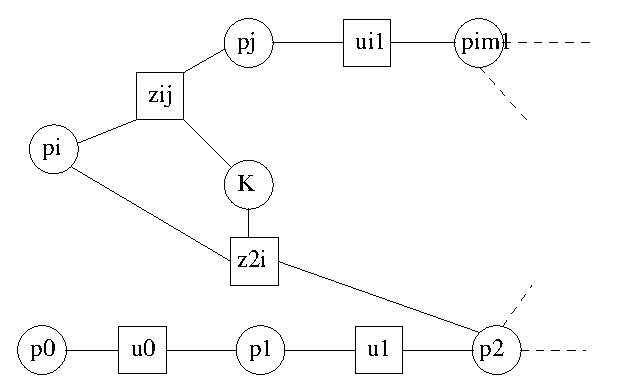
\includegraphics{pics/hgraph.eps}
\caption{This example illustrates how to represent an objective
  function by a hyper-graph. Here we illustrate a portion of a small
  SLAM problem~\cite{konolige10iros}. In this example we assume that
  where the measurement functions are governed by some unknown
  calibration parameters $\mathbf{K}$. The robot poses are represented
  by the variables $\bp_{1:n}$. These variables are connected by
  constraints $\bz_{ij}$ depicted by the square boxes. The constraints
  arise, for instance, by matching nearby laser scans \emph{in the
    laser reference frame}. The relation between a laser match and a
  robot pose, however, depends on the position of the sensor on the
  robot, which is modeled by the calibration parameters
  $\mathbf{K}$. Conversely, subsequent robot poses are connected by
  binary constraints $\bu_{k}$ arising from odometry
  measurements. These measurements are made in the frame of the robot
  mobile base.}
\label{fig:graph-example}
\end{figure}

\section{Least Squares Optimization}
If a good initial guess $\breve{\bx}$ of the parameters is known, a
numerical solution of \eqref{eq:toMinimize} can be obtained by using
the popular Gauss-Newton or Levenberg-Marquardt
algorithms~\cite[\S15.5]{Press92Book}.  The idea is to approximate the
error function by its first order Taylor expansion around the current
initial guess $\breve{\bx}$
\begin{eqnarray}
\be_{k}(\breve{\bx}_k + \bDeltax_k) &=& \be_{k}(\breve{\bx} + \bDeltax)\\
&\simeq& \ec_{k} + \bJ_{k} \bDeltax.
\label{eq:taylor}
\end{eqnarray}
Here $\bJ_{k}$ is the Jacobian of $\be_{k}(\bx)$ computed in
$\breve{\bx}$ and $\ec_{k} \defeq \be_{k}(\breve{\bx})$.
Substituting \eqref{eq:taylor} in the error terms $\bF_{k}$ of
\eqref{eq:sumOfFactors}, we obtain

\vspace{-3.5mm}
{\small
\begin{eqnarray}
\lefteqn{\bF_{k}(\breve{\bx} + \bDeltax) }\\
&=&  \be_{k}(\breve{\bx} + \bDeltax)^T \bOmega_{k} \be_{k}(\breve{\bx} + \bDeltax)  \\
\label{eq:errorQuad1}
             &\simeq& \left(\ec_{k} + \bJ_{k} \bDeltax \right)^T \bOmega_{k} \left(\ec_{k} + \bJ_{k} \bDeltax \right)  \\
\label{eq:errorQuad2}
             &=& \underbrace{\ec_{k}^T \bOmega_{k}\ec_{k}}_{\mathrm{c}_{k}} + 2 \underbrace{\ec_{k}^T \bOmega_{k} \bJ_{k}}_{\bb_{k}} \bDeltax +
 \bDeltax^T \underbrace{\bJ_{k}^T \bOmega_{k}\bJ_{k}}_{\bH_{k}} \bDeltax \\
             &=&\mathrm{c}_{k} + 2 \bb_{k} \bDeltax + \bDeltax^T \bH_{k} \bDeltax
\label{eq:errorQuad}
\end{eqnarray}
} 
With this local approximation, we can rewrite the function
$\bF(\bx)$ given in \eqref{eq:sumOfFactors} as

\vspace{-3.5mm}
{\small
\begin{eqnarray}
\bF(\breve{\bx} + \bDeltax) &=& \sum_{k \in\mathcal{C}} \bF_{k}(\breve{\bx} + \bDeltax) 
\label{eq:optNetwork0}\\
                      &\simeq& \sum_{k \in\mathcal{C}} \mathrm{c}_{k} + 2 \bb_{k} \bDeltax + \bDeltax^T \bH_{k} \bDeltax
\label{eq:optNetwork1}\\
                      &=&\mathrm{c} + 2 \bb^T \bDeltax + \bDeltax^T \bH \bDeltax. 
\label{eq:optNetwork2}
\end{eqnarray}
} The quadratic form in \eqref{eq:optNetwork2} is obtained from
\eqref{eq:optNetwork1} by setting $\mathrm{c}=\sum \mathrm{c}_{k}$,
$\bb=\sum \bb_{k}$ and $\bH=\sum \bH_{k}$. It can be minimized in
$\bDeltax$ by solving the linear system
\begin{eqnarray}
       \bH\,\bDeltax^* &=& - \bb. 
\label{eq:oneLinearIteration}
\end{eqnarray}
The matrix $\bH$ is the information matrix of the system and is sparse
by construction, having non-zeros only between blocks connected by a
constraint.  Its number of non-zero blocks is twice the number of
constrains plus the number of nodes. This allows to solve
\eqref{eq:oneLinearIteration} with efficient approaches like sparse
Cholesky factorization or Preconditioned Conjugate Gradients (PCG). An
highly efficient implementation of sparse Cholesky factorization can
be found in publicly available packages like CSparse~\cite{csparse} or
CHOLMOD~\cite{cholmod}.  The linearized solution is then obtained by
adding to the initial guess the computed increments
\begin{eqnarray}
  \bx^*&=&\breve{\bx}+\bDeltax^*.
\label{eq:linearPropagation}
\end{eqnarray}
The popular Gauss-Newton algorithm iterates the linearization in
\eqref{eq:optNetwork2}, the solution in \eqref{eq:oneLinearIteration}
and the update step in \eqref{eq:linearPropagation}. In every
iteration, the previous solution is used as linearization point and as
initial guess.

The Levenberg-Marquardt (LM) algorithm is a nonlinear variant to Gauss-Newton that introduces 
a damping factor and backup actions to control the convergence.
Instead of solving directly Eq.~\ref{eq:oneLinearIteration}
LM solves a damped version of it
\begin{eqnarray}
       (\bH +\lambda \bI)\,\bDeltax^* &=& - \bb. 
\label{eq:oneLinearIterationLevenberg}
\end{eqnarray}
Here $\lambda$ is a damping factor: the larger $\lambda$ is the
smaller are the $\bDeltax$. This is useful to control the step size in
case of non-linear surfaces.  The idea behind the LM algorithm is to
dynamically control the damping factor.  At each iteration the error
of the new configuration is monitored.  If the new error is lower than
the previous one, lambda is decreased for the next iteration.
Otherwise, the solution is reverted and lambda is increased.
For a more detailed explanation of the LM algorithm implemented in our package
we refer to~\cite{lourakis2009toms}.

The procedures described above are a general approach to multivariate
function minimization. The general approach, however, assumes that the
space of parameters $\bx$ is Euclidean, which is not valid for several
problems like SLAM or bundle adjustment. This may lead to sub-optimal
solutions. In the remainder of this section we discuss first the
general solution when the space of the parameters is Euclidean, and
subsequently we extend this solution to more general non-Euclidean
spaces.

\section{Considerations about the Structure of the Linearized System}
According to \eqref{eq:optNetwork2}, the matrix $\bH$ and the vector
$\bb$ are obtained by summing up a set of matrices and vectors, one
for every constraint.  If we set $\bb_{k}=\bJ_{k}^T \bOmega_{k}
\ec_{k}$ and $\bH_{k}= \bJ_{k}^T \bOmega_{k}\bJ_{k}$ we can
rewrite $\bH$ and $\bb$ as
\begin{eqnarray}
  \bb&=&\sum_{k \in\mathcal{C}} \bb_{ij}\\ 
  \bH&=&\sum_{k \in\mathcal{C}} \bH_{ij}. \label{eq:addendTerm}
\end{eqnarray}
Every constraint will contribute to the system with an addend
term. The \emph{structure} of this addend depends on the Jacobian of
the error function.  Since the error function of a constraint depends
only on the values of the nodes $\bx_i \in \bx_k$, the Jacobian in
\eqref{eq:taylor} has the following form:
\begin{eqnarray}
\bJ_{k} &=& \left(\bZero \cdots \bZero \; \bJ_{k_1} \; \cdots \; \bJ_{k_i} \;\cdots \bZero\; \cdots\;  \bJ_{k_q} \bZero \cdots \bZero \right).
\label{eq:jacExpanded}
\end{eqnarray}
Here $\bJ_{k_i}= \frac{\partial \be(\bx_k)}{\partial \bx_{k_i}}$ are the
derivatives of the error function with respect to the nodes connected
by the $k^\mathrm{th}$ hyper-edge, with respect to the parameter block
$\bx_{k_i} \in \bx_k$.

From \eqref{eq:errorQuad2} we obtain the following structure for the block matrix $\bH_{ij}$:
\begin{eqnarray}
\bH_{k}&=&\left(
\begin{array}{cccccccc}
\ddots & & & & & & &\\
& \bJ_{k_1}^T \bOmega_{k} \bJ_{k_1} & \cdots & \bJ_{k_1}^T \bOmega_{k} \bJ_{k_i} & \cdots & \bJ_{k_1}^T \bOmega_{k} \bJ_{k_q} &\\
& \vdots & & \vdots & & \vdots & \\
& \bJ_{k_i}^T \bOmega_{k} \bJ_{k_1} & \cdots & \bJ_{k_i}^T \bOmega_{k} \bB_{k_i} & \cdots & \bJ_{k_i}^T \bOmega_{k} \bJ_{k_q} & \\
& \vdots & & \vdots & & \vdots & \\
& \bJ_{k_q}^T \bOmega_{k} \bJ_{k_1} & \cdots & \bJ_{k_q}^T \bOmega_{k} \bB_{k_i} & \cdots & \bJ_{k_q}^T \bOmega_{k} \bJ_{k_q} & \\
& &&&&&& \ddots \\
\end{array}
\right) \\
\bb_{k}&=&\left(
\begin{array}{c}
\vdots\\
\bJ_{k_1} \bOmega_{k} \ec_{k}\\
\vdots\\
\bJ_{k_i}^T \bOmega_{k} \ec_{k}\\
\vdots\\
\bJ_{k_q}^T \bOmega_{k} \ec_{k}\\
\vdots\\
\end{array}
\right) 
\end{eqnarray}
For simplicity of notation we omitted the zero blocks.  The reader
might notice that the block structure of the matrix $\bH$ is the
adjacency matrix of the hyper graph.  Additionally the Hessian $\bH$
is a symmetric matrix, since all the $\bH_k$ are symmetric. A single
hyper-edge connecting $q$ vertices will introduce $q^2$ non zero
blocks in the Hessian, in correspondence of each pair $\left<
\bx_{k_i}, \bx_{k_j} \right>$, of nodes connected.


\section{Least Squares on Manifold}
\label{sec:manifold}

To deal with parameter blocks that span over a non-Euclidean spaces,
it is common to apply the error minimization on a manifold.  A
manifold is a mathematical space that is not necessarily Euclidean on
a global scale, but can be seen as Euclidean on a local
scale~\cite{Lee2003SmoothManifolds}.

For example, in the context of SLAM problem, each parameter block
$\bx_i$ consists of a translation vector $\bt_i$ and a rotational
component $\balpha_i$. The translation~$\bt_i$ clearly forms a Euclidean
space. In contrast to that, the rotational components~$\balpha_i$ span
over the non-Euclidean 2D or 3D rotation group $SO(2)$ or $SO(3)$.  To
avoid singularities, these spaces are usually described in an
over-parameterized way, e.g., by rotation matrices or quaternions.
Directly applying \eqref{eq:linearPropagation} to these
over-parameterized representations breaks the constraints induced by the
over-parameterization. The over-parameterization results in additional
degrees of freedom and thus introduces errors in the solution.  To
overcome this problem, one can use a minimal representation for the
rotation (like Euler angles in 3D). This, however, is then subject to
singularities.

An alternative idea is to consider the underlying space as a manifold
and to define an operator $\boxplus$ that maps a local variation
$\bDeltax$ in the Euclidean space to a variation on the manifold,
$\bDeltax\mapsto\bx\boxplus\bDeltax$.  We refer the reader to
\cite[\S1.3]{hertzberg08diplom} for more mathematical details. With
this operator, a new error function can be defined as
\begin{eqnarray}
\breve \be_{k}(\bTDeltax_k) &\defeq&
  \be_{k}(\bbx_k \boxplus \bTDeltax_k) \\
  &=& \be_{k}(\bbx \boxplus \bTDeltax) \label{eq:manifoldTaylor0}
  \simeq \breve \be_{k} + \tilde \bJ_{k} \bTDeltax,
\label{eq:manifoldTaylor}
\end{eqnarray}
where $\bbx$ spans over the original over-parameterized space, for
instance quaternions. The term $\bTDeltax$ is a small increment around
the original position $\bbx$ and is expressed in a minimal
representation. A common choice for $SO(3)$ is to use the vector part
of the unit quaternion.
%
In more detail, one can represent the increments $\bTDeltax$ as 6D vectors
$\bTDeltax^T = ( {\bDelta\tilde\bt}^T \, {\bqTilde}^T)$,
where $\bDelta \tilde \bt$ denotes the translation and $\bqTilde^T
= ( \Delta q_x \, \Delta q_y \, \Delta q_z)^T$ is the
vector part of the unit quaternion representing the 3D rotation.  Conversely, $\bbx^T=(
\breve \bt^T \, \breve \bq^T)$ uses a quaternion $\breve \bq$ to
encode the rotational part.  Thus, the operator $\boxplus$ can be
expressed by first converting $\bDelta \tilde \bq$ to a full quaternion $\bDelta
\bq$ and then applying the transformation $\bDelta \bx ^T = ( \bDelta
\bt^T \, \bDelta \bq^T)$ to $\bbx$.  In the equations
describing the error minimization, these operations can nicely be
encapsulated by the $\boxplus$ operator.  The Jacobian $\tilde
\bJ_{k}$ can be expressed by
\begin{eqnarray}
\tilde \bJ_{k} &=& \left. \frac{\partial \be_{k}(\breve{\bx} \boxplus \bTDeltax)} {\partial \bTDeltax} \right|_{\bTDeltax=\bZero}.
\label{eq:manifoldJacobian}
\end{eqnarray}
Since in the previous equation $\breve{\be}$ depends only on $\bTDeltax_{k_i} \in \bTDeltax_{k}$ we can further expand it as follows:
\begin{eqnarray}
\tilde \bJ_{k} &=& 
\left. 
\frac{\partial \be_{k}(\breve{\bx} \boxplus \bTDeltax)} {\partial \bTDeltax} \right|_{\bTDeltax=\bZero}\\
&=& \left(\bZero \cdots \bZero \; \tilde \bJ_{k_1} \; \cdots \; \tilde \bJ_{k_i} \;\cdots \bZero\; \cdots\;  \tilde \bJ_{k_q} \bZero \cdots \bZero \right).
\label{eq:manifoldJacobianSparse}
\end{eqnarray}
With a straightforward extension of notation, we set
\begin{equation}
\tilde \bJ_{k_i} = \left. \frac{ \partial \be_{k}(\breve{\bx} \boxplus \bTDeltax)}{\partial \bTDeltax_{k_i}} \right|_{\bTDeltax=\bZero}
\end{equation}

%% Using the rule on the partial derivatives and exploiting the fact
%% that the Jacobian is evaluated in $\bTDeltax=\bZero$, the non-zero
%% blocks become:
%% \begin{eqnarray}
%% \frac{\partial \be_{k}(\breve{\bx_k} \boxplus \bTDeltax_k)} {\partial \bTDeltax_i} &=& 
%% \underbrace{\frac{\partial \be_{k}(\breve{\bx})} {\partial \breve{\bx}_i}}_{\bJ_{k_i}} 
%% \cdot
%% \left.
%% \underbrace{
%% \frac{\breve{\bx}_{k_i} \boxplus \bTDeltax_{k_i}} {\partial \bTDeltax_{k_i}}
%% }_{\bM_{k_i}}
%% \right|_{\bTDeltax=\bZero}
%% \label{eq:manifoldJacobianBlocks}
%% \end{eqnarray}
%% Accordingly, one can easily derive from the a Jacobian \emph{not} defined on a manifold
%% of Eq.~\ref{eq:jacExpanded} a Jacobian on a manifold just by multiplying its non-zero blocks
%% by the derivative of the $\boxplus$ operator computed in $\breve{\bx_i}$ and $\breve{\bx_j}$.
%% Let the Jacobians of $\boxplus$ be denoted by $\bM_{k_i}$. By using the notation in 
%% Eq.~\ref{eq:jacExpanded} we can rewrite Eq.~\ref{eq:manifoldJacobian} as
%% \begin{eqnarray}
%% \tilde \bJ_{ij} &=& 
%% \left(\bZero \cdots \bZero \; \bJ_{k_1} \bM_{k_1} \; \cdots \; \bJ_{k_i} \bM_{k_i} \;\cdots \bZero\; \cdots\; \bJ_{k_q}\bM_{k_q} \bZero \cdots \bZero \right).
%% \label{eq:jacManExpanded}
%% \end{eqnarray}

With a straightforward extension of the notation, we can insert
\eqref{eq:manifoldTaylor} in \eqref{eq:errorQuad1} and
\eqref{eq:optNetwork0}. This leads to the following increments:
\begin{eqnarray}
       \tilde \bH \, \bTDeltax^* &=& - \tilde \bb .
\label{eq:oneLinearManifoldIteration}
\end{eqnarray}
Since the increments $\bTDeltax^*$ are computed in the local Euclidean
surroundings of the initial guess $\breve{\bx}$, they need to be
re-mapped into the original redundant space by the $\boxplus$
operator. Accordingly, the update rule of \eqref{eq:linearPropagation}
becomes
\begin{eqnarray}
  \bx^*& =& \breve{\bx} \boxplus \bTDeltax^*.
\label{eq:manifoldPropagation}
\end{eqnarray}
In summary, formalizing the minimization problem on a manifold consists
of first computing a set of increments in a local Euclidean
approximation around the initial guess by
\eqref{eq:oneLinearManifoldIteration}, and second accumulating the
increments in the global non-Euclidean space by
\eqref{eq:manifoldPropagation}.  Note that the linear system computed on
a manifold representation has the same structure like the linear system
computed on an Euclidean space.  One can easily derive a manifold
version of a graph minimization from a non-manifold version, only by
defining an $\boxplus$ operator and its Jacobian $\tilde \bJ_{k_{i}}$
w.r.t.  the corresponding parameter block.  In \gopt{} we provide tools
for numerically computing the Jacobians on the manifold space.  This
requires the user to implement the error function and the $\boxplus$
operator only. As a design choice, we do not address the non-manifold
case since it is already contained in the manifold one.  However, to
achieve the maximum performances and accuracy we recommend the user to
implement analytic Jacobians, once the system is functioning with the
numeric ones.

\section{Robust Least Squares\label{sec:robust_kernel}}
Optionally, the least squares optimization can be robustified.
Note, that the error terms in Eq.~\ref{eq:sumOfFactors}  have the following form:
\begin{eqnarray}
\bF_k = \be_k^T\Omega_k \be_k = \rho_2\left(\sqrt{\be_k^T\Omega_k \be_k}\right) \quad \text{with} \quad \rho_2(x):=x^2.
\end{eqnarray}
Thus, the error vector $\be_k$ has quadratic influence on $\bF$, 
so that a single potential outlier would have major negative impact.
In order be more outlier robust, the quadratic error function $\rho_2$
can be replaced by a more robust cost function which weighs large errors less. 
In \gopt, the Huber cost function $\rho_H$ can be used
\begin{eqnarray}
\rho_H(x) := \begin{cases}
                 x^2         & \text{if } |x|<b\\
                  2b |x| - b^2          & \text{else},
   \end{cases}
\end{eqnarray}
which is quadratic for small $|x|$ but linear for large $|x|$. Compared to other,
even more robust cost functions, the Huber kernel has to advantage that it is
still convex and thus does not introduce new local minima in $\bF$~\cite[pp.616]{Hartley:Zisserman:Book2004}.
In practice, we do not need to modify Eq.~$\ref{eq:sumOfFactors}$. Instead, the following scheme 
is applied. First the  error $\be_k$ is computed as usual. Then, $\be_k$ is replaced by 
a weighted version $w_k\be_k$ such that 
\begin{eqnarray}
(w_k\be_k)^T\Omega_k (w_k\be_k) = \rho_H\left(\sqrt{\be_k^T\Omega_k \be_k}\right).
\end{eqnarray}
Here, the weights $w_k$ are calculated as follows
\begin{eqnarray}
w_k = \frac{\sqrt{\rho_H\left(||\be_k||_\Omega \right)}}{||\be_k||_\Omega } \quad \text{with} \quad ||\be_k||_\Omega := \sqrt{\be_k^T\Omega_k \be_k}.
\end{eqnarray}
In \gopt, the user has fine-grained control and can enable/disable the robust cost function for each edge individually (see Section~\ref{sec:error}).




\section{Library Overview}
From the above sections it should be clear that a graph-optimization problem is entirely defined by:
\begin{itemize}
\item The types of the vertices in the graph (that are the parameters blocks $\{\bx_i\}$. 
  For each of those one has to specify:
  \begin{itemize}
    \item the domain $\Dom(\bx_i)$ of the internal parameterization, 
    \item the domain $\Dom(\bDeltax_i)$ of the increments $\bDeltax_i$,
    \item $\boxplus: \Dom(\bx_i) \times \Dom(\bDeltax_i) \rightarrow \Dom(\bx_i)$ that 
      applies the increment $\bDeltax_i$ to the previous solution $\bx_i$.
  \end{itemize}
\item the error function for every type of hyper-edge
  $\be_{k}:\Dom(\bDeltax_{k_1}) \times \Dom(\bDeltax_{k_2}) \times \dots \times
  \Dom(\bDeltax_{k_q}) \rightarrow \Dom(\bz_{k})$ that should be zero when
  the perturbated estimate $\bx_{k} \boxplus \bDeltax_{k}$ perfectly satisfies the constraint $\bz_{k}$.
\end{itemize}
By default the Jacobians are computed numerically by our
framework. However to achieve the maximum performances in a specific
implementation one can specify the Jacobian of the error functions and
of the manifold operators.

In the reminder we will shortly discuss some basic concepts to use and
extend \gopt.  This documentation is by no means complete, but it is
intended to help you browsing the automatically generated
documentation. To better visualize the interplay of the components of
\gopt{} we refer to the class diagram of Figure~\ref{fig:classes}.
\begin{figure}
\centering
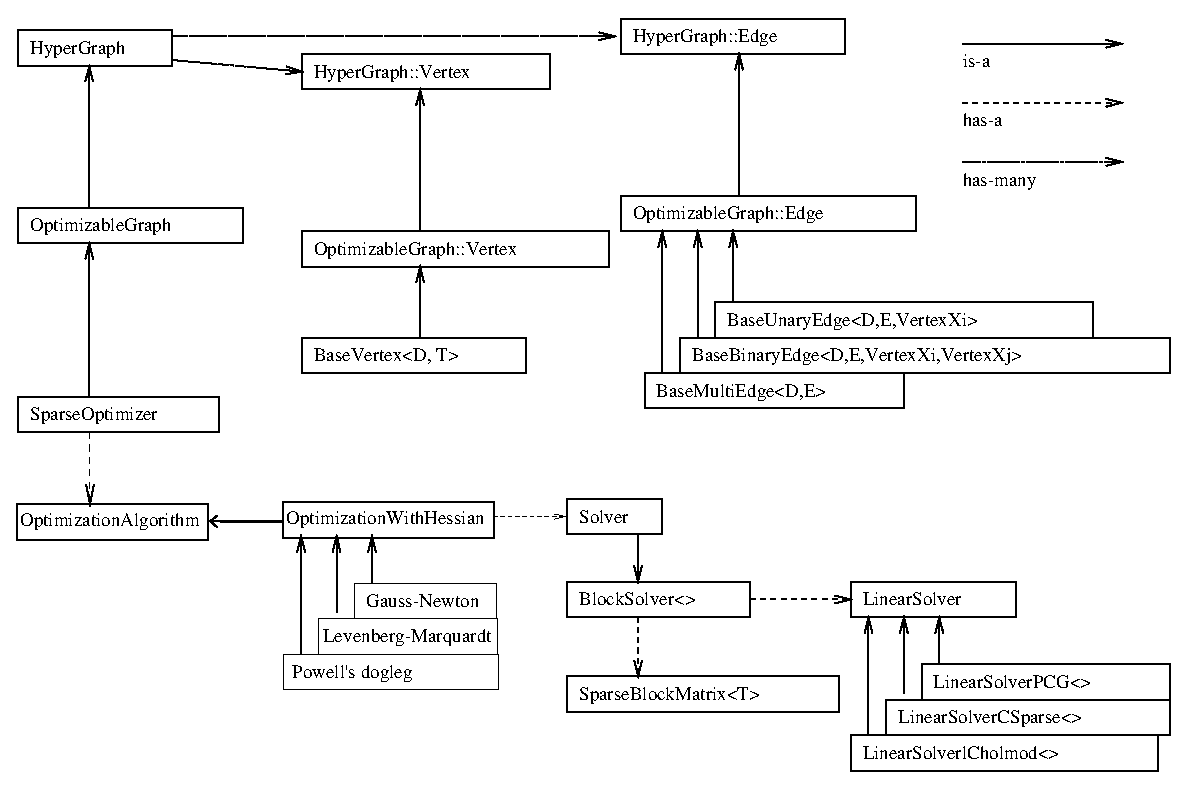
\includegraphics[width=0.7\columnwidth]{pics/classes.eps}
\caption{Class diagram of \gopt{}.}
%% TODO update by adding OptimizationAlgorithm
\label{fig:classes}
\end{figure}

\subsection {Representation of an Optimization Problem}
\label{sec:representation}
All in all our system utilizes a generic hyper-graph structure to
represent a problem instance (defined in \verb+hyper_graph.h+).  This
generic hyper graph is specialized to represent an optimization
problem by the class \verb+OptimizableGraph+, defined in
\verb+optimizable_graph.h+.  Within the \verb+OptimizableGraph+ the
inner classes \verb+OptimizableGraph::Vertex+ and
\verb+OptimizableGraph::Edge+ are used to represent generic hyper
edges and hyper vertices.  Whereas the specific implementation might
be done by directly extending these classes, we provided a template
specialization that implements automatically most of the methods that
are mandatory for the system to work.

These classes are \verb+BaseVertex+ and \verb+BaseUnaryEdge+,
\verb+BaseBinaryEdge+ and \verb+BaseMultiEdge+. 
\begin{description}
\item \verb+BaseVertex+ templatizes the dimension of a parameter block
  $\bx_i$ and of the corresponding manifold $\bDeltax_i$, thus it can 
  use blocks of memory whose layout is known at compile-time (means
  efficiency). Furthermore, it implements some mapping operators to
  store the Hessian and the parameter blocks of the linearized
  problem, and a stack of previous values that can be used to
  save/restore parts of the graph.  The method \verb+oplusImpl(double* v)+
  that applies the perturbation $\bDeltax_i$ represented by \verb+v+,
  to the member variable \verb+_estimate+ should be implemented. This
  is the $\boxplus$ operator. Additionally,
  \verb+setToOriginImpl()+ that should set the internal state of the vertex
  to $\bZero$ has to specified.

\item \verb+BaseUnaryEdge+ is a template class to model a unary
  hyper-edge, which can be used to represent a prior. It offers for
  free the calculation of the Jacobians, via an implementation of the
  \verb+linearizeOplus+ method. It requires to specify the types of
  the (single) vertex $\bx_i$, and type and dimension of the error 
  $\be(\bx_k)$ as template parameters.  The function
  \verb+computeError+ that stores the result of the error $\be(\bx_k)$ in the
  member \verb+Eigen::Matrix _error+ should be implemented.

\item \verb+BaseBinaryEdge+ is a template class that models a binary
  constraint, namely an error function in the form $\be_k(\bx_{k_1},
  \bx_{k_2})$. It offers the same facilities of \verb+BaseUnaryEdge+, and it
  requires to specify the following template parameters: the type of the nodes
  $\bx_{k_1}$ and $\bx_{k_2}$  and the  type and the dimension of the measurement. 
  Again, it implements the numeric Jacobians via
  a default implementation of the \verb+linearizeOplus+ method.
  Again, the \verb+computeError+ should be implemented in a derived class.

\item \verb+BaseMultiEdge+ is a template class that models a
  multi-vertex constraint in the form of $\be_k(\bx_{k_1}, \bx_{k_2},
  \ldots, \bx_{k_q})$. It offers the same facilities of the types
  above, and it requires to specify only the type and dimension of the
  measurement as template parameters. The specialized class should
  take care of resizing the connected vertices to the correct size
  $q$.  This class relies on a dynamic memory, since too many
  parameters are unknown, and if you need of an efficient
  implementation for a specific problem you can program it yourself.
  Numeric Jacobian comes for free, but you should implement the
  \verb+computeError+ in a derived class, as usual
\end{description}

In short, all you need to do to define a new problem instance is to
derive a set of classes from those above listed, one for each type of
parameter block and one for each type of (hyper)edge. Always try to
derive from the class which does the most work for you.  If you want to
have a look at a simple example look at \verb+vertex_se2+ and
\verb+edge_se2+. Those two types define a simple 2D graph SLAM
problem, like the one described in many SLAM papers.

\begin{lstlisting}[float,label=lst:inittypes,caption=Registering types
  by a constructor from a library]
#include "g2o/core/factory.h"

namespace g2o {
  G2O_REGISTER_TYPE_GROUP(slam2d);

  G2O_REGISTER_TYPE(VERTEX_SE2, VertexSE2);
  G2O_REGISTER_TYPE(VERTEX_XY, VertexPointXY);

  // ...
}
\end{lstlisting}

Of course, for every type you construct you should define also the
\verb+read+ and \verb+write+ functions to read and write your data to a
stream.  Finally, once you define a new type, to enable the loading and
the saving of the new type you should ``register'' it to a factory.
This is easily done by assigning a string tag to a new type, via the
\verb+registerType+ function. This should be called once before
all files are loaded.

To this end, \gopt{} provides an easy macro to carry out the registration of the
class to the factory.  See Listing~\ref{lst:inittypes} for an example,
the full example can be found in \verb+types_slam2d.cpp+.  The first
parameter given to the macro \verb+G2O_REGISTER_TYPE+ specifies the tag
under which a certain vertex / edge is known. \gopt\ will use this
information while loading files and for saving the current graph into a
file. In the example given in Listing~\ref{lst:inittypes} we register
the tags \verb+VERTEX_SE2+ and \verb+EDGE_SE2+ with the classes
\verb+VertexSE2+ and \verb+EdgeSE2+, respectively.

Furthermore, the macro \verb+G2O_REGISTER_TYPE_GROUP+ allows to declare
a type group. This is necessary if we use the factory to construct the
types and we have to enforce that our code is linked to a specific type
group. Otherwise the linker may drop our library, since we do not
explicitly use any symbol provided by the library containing our type.
Declaring the usage of a specific type library and hence enforcing the
linking is done by the macro called \verb+G2O_USE_TYPE_GROUP+.

\subsection{Construction and Representation of the Linearized Problem}
The construction and the solution can be separated into individual
steps which are iterated.
\begin{itemize}
  \item Initialization of the optimization (only before the first
    iteration).
  \item Computing the error vector for each constraint.
  \item Linearize each constraint.
  \item Build the linear system.
  \item Updating the Levenberg-Marquardt damping factor.
\end{itemize}

Within the following sections we will describe the steps.

\subsubsection{Initialization}
The class \verb+SparseOptimizer+ offers several methods to initialize
the underlying data structure. The methods
\verb+initializeOptimization()+ either takes a subset of vertices or a
subset of edges which will be considered for the next optimization runs.
Additionally, all vertices and edges can be considered for optimization.
We refer to the vertices and edges currently considered as \emph{active}
vertices and edges, respectively.

Within the initialization procedure, the optimizer assigns a temporary
index to each active vertex. This temporary index corresponds to the
block column / row of the vertex in the Hessian. Some of the vertices
might need to be kept fixed during the optimization, to resolve
arbitrary degrees of freedom (gauge freedom). This can be done by
setting the \verb+_fixed+ attribute of a vertex.

\subsubsection{Compute error\label{sec:error}}
The \verb+computeActiveErrors()+ function takes the current estimate of
the active vertices and for each active edge calls
\verb+computeError()+ for computing the current error vector. Using
the base edge classes described in Section~\ref{sec:representation} 
the error should be cached in the member variable \verb+_error+.

 If \verb+robustKernel()+ is set to true for a particular active edge,
\verb+robustifyError()+ is called and \verb+_error+ is robustified 
as described in Section~\ref{sec:robust_kernel}.

\subsubsection{Linearizing the system}
Each active edge is linearized by calling its
\verb+linearizeOplus()+ function. Again the Jacobians can be cached by
member variables provided by the templatized base classes described in 
Section~\ref{sec:representation}. If the \verb+linearizeOplus()+
function is not re-implemented the Jacobian will be computed
numerically as follows:
\begin{eqnarray}
  \tilde \bJ_k^{\bullet l} = \frac{1}{2\delta} \left(
  \be_k (\bx_k \boxplus \delta\mathbf{1}_l)
  -
  \be_k (\bx_k \boxplus -\delta\mathbf{1}_l)
  \right),
  \label{eqn:jacobiannumeric}
\end{eqnarray}
where $\delta > 0$ is a small constant ($10^{-9}$ in our
implementation) and $\mathbf{1}_l$ is the unit vector along dimension
$l$. Note that we only store and calculate the non-zero entries of
$\tilde \bJ_k$ that have not been fixed during the initialization.

\subsubsection{Building the system}
For each active edge the addend term for Eq.~\ref{eq:addendTerm} is
computed by multiplying the corresponding blocks of the Jacobians and
the information matrix of the edge. The addend term is calculated in
each edge by calling \verb+constructQuadraticForm()+.

\subsubsection{Updating Levenberg-Marquardt}
As illustrated in \eqref{eq:oneLinearIterationLevenberg} the
Levenberg-Marquardt algorithm requires updates to the linear system.
However, only the elements along the main diagonal need to be modified.
To this end, the methods \verb+updateLevenbergSystem(double lambda)+ and
\verb+recoverSystem(double lambda)+ of the \verb+Solver+ class apply the
modifications by respectively adding or subtracting $\lambda$ along the
main diagonal of $\bH$.

\subsection{Solvers}
A central component of these least-squares approaches is the solution
of the linear system $\tilde \bH \, \bTDeltax^* = - \tilde \bb$. To
this end there are several approaches available, some of them exploit
the known structure of certain problems and perform intermediate
reductions of the system, like by applying the Schur complement to a
subset of variables.  In \gopt{} we do not select any particular solver,
but we rely on external libraries.  To this end, we decouple these
\emph{structural} operations (like the Schur complement)
from the solution of the linear system.

The construction of the linear problem from the Jacobian matrices and the error vectors
in the hyper-graph elements are controlled by a so-called \verb+Solver+ class.
To use a specific factorization of the system, the user has to extend the
\verb+Solver+ class, and to implement the virtual functions. 
Namely a solver should be able to extract from an
hyper-graph the linear system, and to return a solution.  This is
done in several steps: at the beginning of the optimization the
function \verb+initializeStructure+ is called, to allocate the
necessary memory that will be overwritten in the subsequent
operations. This is possible since the structure of the system does
not change between iterations. Then the user should provide means to
access to the increment vector $\bTDeltax$ and $\tilde \bb$, via the
functions \verb+b()+ and \verb+x()+. To support Levenberg-Marquardt
one should also implement a function to perturb the Hessian with the
$\lambda \bI$ term. This function is called
\verb+setLambda(double lambda)+ and needs to be implemented by the
specific solver.

We provide a templatized implementation of the solver class, the
\verb+BlockSolver<>+ that stores the linear system in a
\verb+SparseBlockMatrix<>+ class. The \verb+BlockSolver<>+ implements
also the Schur complement, and relies on another abstract class, the
\verb+LinearSolver+ to solve the system.
An implementation of the linear solver does the actual work
of solving the (reduced) linear system, and has to implement a few methods.
In this release of \gopt{} we provide linear solvers that use respectively
preconditioned gradient descent, CSparse, and CHOLMOD.


\subsection{Actions}
To the extent of \gopt{}, the entities stored in a hyper-graph have a
pure mathematical meaning. They either represent variables to be
optimized (vertices), or they encode optimization constraints.
However, in general these variables are usually related to more
``concrete'' objects, like laser scans, robot poses, camera parameters
and so on.  Some variable type may support only a subset of feasible
operations.  For instance it is possible to ``draw'' a robot pose, but
it is not possible to ``draw'' the calibration parameters.  More in
general we cannot know a priori the kind of operations that will be
supported by the user types of \gopt.  However, we want to design a set
of tools and of functions that rely on certain operations. These include,
for instance viewers, or functions to save/load the graph in a specific format.

A possibility to do this would be to ``overload'' the base classes of
the hyper-graph elements (vertices and edges) with many virtual
functions, one for each of the functionality we want to support.  This
is of course not elegant, because we would need to patch the base
classes with the new function every time something new is added.
Another possibility would be to make use of the multiple inheritance
of C++, and to define an abstract ``drawable'' object, on which the
viewer operates.  This solution is a bit better, however we cannot
have more than one ``drawing'' function for each object.

The solution used in \gopt{} consists in creating a library of
function objects that operate on the elements (vertices or edges) of
the graph.  One of these function objects is identified by a function
name and by a type on which it operates.  These function objects can
be registered into an action library.  Once these objects are loaded
in the action library it is possible to call them on a graph.  These
functionalities are defined in \verb+hyper_graph_action.h+.  It is
common to register and create the actions when defining the types for
the edges and the vertices.  You can see many examples in
\verb+types_*/*.h+.

\section{\gopt\ Tools}
\gopt\ comes with two tools which allow to process data stored in
files. The data can be loaded from a file and stored again after
processing. In the following we will give a brief introduction to these
tools, namely a command line interface and a graphical user interface.

\subsection{\gopt\ Command Line Interface}

\verb+g2o+ is the command line interface included in \gopt. It
allows to optimize graphs stored in files and save the result back to a
file. This allows a fast prototyping of optimization problems, as it is
only required to implement the new types or solvers. The \gopt\
distribution includes a data folder which comprises some data files on
which \verb+g2o+ can be applied.

\subsection{\gopt\ Viewer}

\begin{figure}
  \centering
  \includegraphics[width=0.7\columnwidth]{pics/viewer}
  \caption{Graphical interface to \gopt. The GUI allows to select
  different suitable optimizers and perform the optimization.}
  \label{fig:viewer}
\end{figure}

The Graphical User Interface depicted in Figure~\ref{fig:viewer} allows
to visualize the optimization problem. Additionally, the various
parameters of the algorithms can be controlled.

\subsection{\gopt{} incremental}

\gopt{} includes an experimental binary for performing optimization in
an incremental fashion, i.e., optimizing after inserting one or several
nodes along with their measurements. In this case, \gopt{} performs
rank updates on the Hessian matrix to update the linear system. Please
see the \verb+README+ in the \verb+g2o_incremental+ sub-folder for
additional information.

Example for the Manhattan3500 dataset:
\begin{verbatim}
g2o_incremental -i manhattanOlson3500.g2o
\end{verbatim}

\subsection{Plug-in Architecture}

\begin{lstlisting}[float,label=lst:initsolvers,caption=Registering
  solvers by a constructor from a library]
class PCGSolverCreator : public AbstractOptimizationAlgorithmCreator
{
  public:
    PCGSolverCreator(const OptimizationAlgorithmProperty& p) : AbstractOptimizationAlgorithmCreator(p) {}
    virtual OptimizationAlgorithm* construct()
    {
      // create the optimization algorithm
      // see g2o/solver_pcg/solver_pcg.cpp for the details
    }
};

G2O_REGISTER_OPTIMIZATION_LIBRARY(pcg);

G2O_REGISTER_OPTIMIZATION_ALGORITHM(gn_pcg, new PCGSolverCreator(OptimizationAlgorithmProperty("gn_pcg", "Gauss-Newton: PCG solver using block-Jacobi pre-conditioner (variable blocksize)", "PCG", false, Eigen::Dynamic, Eigen::Dynamic)));

G2O_REGISTER_OPTIMIZATION_ALGORITHM(gn_pcg3_2, new PCGSolverCreator(OptimizationAlgorithmProperty("gn_pcg3_2", "Gauss-Newton: PCG solver using block-Jacobi pre-conditioner (fixed blocksize)", "PCG", true, 3, 2)));

//...
\end{lstlisting}

Both tools support the loading of types and optimization algorithms at
run-time from dynamic libraries. This is realized as follows. The tools
load from the libs folder all libraries matching ``*\_types\_*'' and
``*\_solver\_*'' to register types and optimization algorithms,
respectively. We assume that by loading the libraries the types and the
algorithms register via their respective constructors to the system.
Listing~\ref{lst:inittypes} shows how to register types to the system
and Listing~\ref{lst:initsolvers} is an example, which shows how to
register an optimization algorithm via the plug-in architecture.

For loading dynamic library containing types or optimization algorithms, we support two
different methods:
\begin{itemize}
  \item The tools recognize the command line switch \verb+-typeslib+
    and \verb+-solverlib+ to load a specific library.
  \item You may specify the environment variables \verb+G2O_TYPES_DIR+
    and \verb+G2O_SOLVER_DIR+ which are scanned at start and libraries
    matching ``*\_types\_*'' and ``*\_solver\_*'' are automatically
    loaded.
\end{itemize}

\section{2D SLAM: An Example}
SLAM is a well known problem in robotics and this acronym stands for
``Simultaneous Localization And Mapping''. The problem can be stated
as follows: given a moving robot equipped with some sensors, we want
to estimate both the map and the pose of the robot in the environment
from the sensor measurements. Usually, the sensors can be classified
in exteroceptive or proprioceptive.  An exteroceptive sensor is a
device that measures quantities relative to the environment where the
robot moves.  Examples of these sensors can be cameras that acquire an
image of the world at a particular location, laser scanners that
measure a set of distances around the robot or accelerometers in
presence of gravity that measure the gravity vector or GPS that derive
a pose estimate by observing the constellation of known satellites.
In contrast, proprioceptive sensors measure the change of the robot's
state (the position), relative to the previous robot position. Example
include odometers, that measure the relative movement of the robot
between two time steps or gyroscopes. In traditional approaches to
SLAM, like EKF these two sensors play a substantially different role
in the system.  The proprioceptive measurements are used to evolve a
set of state variables, while the exteroceptive measurements are used
to correct these estimates, by feeding back the measurement errors.
This is not the case of smoothing methods (like the ones that can be
implemented with \gopt{}), where all measurements are treated in a
substantially similar manner.

A complete solution to SLAM is typically rather complex and involves
processing raw sensor data and determining correspondences between
previously seen parts of the environment and actual measurements (data
association). Describing a complete solution to the problem is out of
the scope of this document.  However, in the reminder we will present a
simplified but meaningful version of the problem that contains all the relevant elements
and that is well suited to be implemented with \gopt.

The scenario is a robot moving on a plane. The robot is equipped
with an odometry sensor that is able to measure the relative movement
of the robot between two time frames and of a ``landmark'' sensor
that is able to measure the position of some environment landmarks
nearby the robot \emph{in the robot reference frame}. One could
implement this landmark detector, for instance, by extracting corners
from a laser scan or by detecting the position of relevant features
from a stereo image pair. A simplification that we make in this
section is that the landmarks are uniquely identifiable. In other
words whenever the robot sees a landmark, it can tell if it is a new
one or if it has already seen it and when.

Clearly both odometers and landmark sensors are affected by noise.  In
principle, if the odometry would not be affected by noise one could
reconstruct the trajectory of the robot simply by chaining the
odometry measurements. However, this is not the case and integrating
the odometry leads to an increasing positioning error that becomes
evident when the robot reenters a known region. In a similar way,
if the robot would have unlimited perception range, it could acquire
all the map in one shot and the position could be retrieved by simple
geometric constructions. Again this is not the case and the robot
perceives the position of the landmarks that are located within a
maximum range. These measurements are affected by a noise, that
usually increases with the distance of a landmark from the robot.

In the remainder of this section we will walk through all essential
steps that are required to characterize a problem within \gopt{}.
These are:
\begin{itemize}
\item identification of the state variables $\bx_i$ and of their domain,
\item characterization of the constraints and identification of the graph structure,
\item choice of the parameterization for the increments $\bTDeltax_i$, and definition of the
$\boxplus$ operator.
\item construction of the error functions $e_k(\bx_k)$.
\end{itemize}

\subsection{Identification of the State Variables}
Figure~\ref{fig:slam} illustrates a fragment of a SLAM graph.  The
robot positions are denoted by the nodes $\bx^\mathrm{s}_t$, while the
landmarks are denoted by the nodes $\bx^\mathrm{l}_i$. We assume that
our landmark sensor is able to detect only the 2D pose of a landmark,
but not its orientation.  In other words the landmarks ``live'' in
$\Re^2$.  Conversely, the robot poses are parameterized by the robot
location $(x,y)$ on the plane and its orientation $\theta$, thus they
belong to the group of 2D transformations $SE(2)$.  More
formally, the nodes of a 2D SLAM graph are of two types
\begin{itemize}
\item Robot positions $\bx^\mathrm{s}_t = ( x^\mathrm{s}_t  \; y^\mathrm{s}_t \; \theta^\mathrm{s}_t)^T \in SE(2)$
\item Landmark positions $\bx^\mathrm{l}_i = ( x^\mathrm{l}_i  \; y^\mathrm{l}_i )^T \in \Re^2$
\end{itemize}

\begin{figure}
\psfrag{p1}{$\bx^\mathrm{s}_1$}
\psfrag{p2}{$\bx^\mathrm{s}_2$}
\psfrag{pt1}{$\bx^\mathrm{s}_{t-1}$}
\psfrag{pt}{$\bx^\mathrm{s}_{t}$}
\psfrag{L1}{$\bx^\mathrm{l}_1$}
\psfrag{L2}{$\bx^\mathrm{l}_2$}
\psfrag{Li1}{$\bx^\mathrm{l}_{i-1}$}
\psfrag{Li}{$\bx^\mathrm{l}_{i}$}
\psfrag{u12}{$\bz^\mathrm{s}_{1,2}$}
\psfrag{utt1}{$\bz^\mathrm{s}_{t-1,t}$}
\psfrag{l11}{$\bz^\mathrm{l}_{1,1}$}
\psfrag{l12}{$\bz^\mathrm{l}_{1,2}$}
\psfrag{lit}{$\bz^\mathrm{l}_{t,i}$}
\psfrag{l1i}{$\bz^\mathrm{l}_{1,i}$}
\psfrag{lti1}{$\bz^\mathrm{l}_{t,i-1}$}
\psfrag{lt1i}{$\bz^\mathrm{l}_{t-1,i-1}$}
\centering
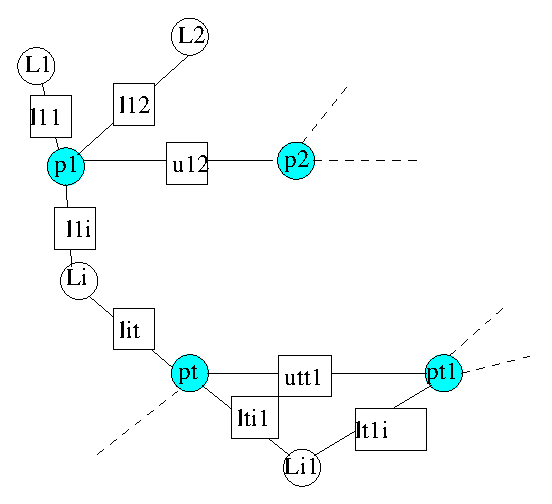
\includegraphics[width=0.8\columnwidth]{pics/slam.eps}
\caption{Graphical representation of a SLAM process. The vertices of
  the graph, depicted with circular nodes, denote either robot poses
  $\bx^\mathrm{s}_*$ or landmarks $\bx^\mathrm{l}_*$. The measurement
  of a landmark from a robot pose is captured by a constraints
  $\bz^{\mathrm{l}}_*$ and odometry measurements connecting subsequent
robot poses are modeled by the constraints $\bz^\mathrm{s}_*$.}
\label{fig:slam}
\end{figure}

\subsection{Modeling of the Constraints}
Two subsequent robot positions $\bx^\mathrm{s}_t$ and
$\bx^\mathrm{s}_{t+1}$ are related by an odometry measurement, that
represent the relative motion that brings the robot from
$\bx^\mathrm{s}_t$ to $\bx^\mathrm{s}_{t+1}$ \emph{measured} by the
odometry. This measurement will be typically slightly different from
the \emph{real} transformation between the two pose because of the
noise affecting the sensors.  Being an odometry measurement, an
Euclidean transformation, it is also a member of $SE(2)$ group.
Assuming the noise affecting the measurement being white and Gaussian,
it can be modeled by an $3 \times 3$ symmetric positive definite
information matrix.  In real applications the entries of this matrix
depend on the motion of the robot.  i.e., the bigger the movement is
the larger the uncertainty will be.
Thus an odometry edge between the nodes $\bx^\mathrm{s}_t$ and
$\bx^\mathrm{s}_{t+1}$ consists of these two entities:
\begin{itemize}
\item $\bz^\mathrm{s}_{t,t+1} \in SE(2)$ that represents the motion
  between the nodes and
\item $\bOmega^\mathrm{s}_{t,t+1} \in \Re^{3 \times 3}$ that represents the
  inverse covariance of the measurement, and thus is symmetric and
  positive definite.
\end{itemize}

If the robot senses a landmark $\bx^\mathrm{l}_i$ from the location
$\bx^\mathrm{s}_t$, the corresponding measurement will be modeled by
an edge going from the robot pose to the landmark. A measurement about
the landmark consists in a point in the $x$-$y$ plane, perceived in the
robot frame. Thus a landmark measurement lives in $\Re^2$ as the
landmarks do. Again, under white Gaussian noise assumption, the
noise can be modeled by its inverse covariance. Accordingly, an edge between
a robot pose and a landmark is parametrized in this way:
\begin{itemize}
\item $\bz^\mathrm{l}_{t,i} \in \Re^2$ that represents position of the landmark
  in the frame expressed by $\bx^\mathrm{s}_t$ and
\item $\bOmega^\mathrm{l}_{t,i} \in \Re^{2 \times 2}$ that represents the inverse
  covariance of the measurement and is SPD.
\end{itemize}

\subsection{Choice of the Parameterization for the Increments}
So far, we defined most of the elements necessary to implement a 2D
SLAM algorithm with \gopt{}.  Namely we characterized the domains of
the variables and the domains of the measurements.  What remains to do
is to define the error functions for the two kinds of edges in our
system and to determine a (possibly smart) parameterization for the
increments.


The landmark positions are parameterized in $\Re^2$, which is already
an Euclidean space. Thus the increments $\bTDeltax^\mathrm{l}_i$ can live in the same space and the
 $\boxplus$ operator can be safely chosen as the vector sum:
\begin{eqnarray}
  \bx^\mathrm{l}_i \boxplus \bTDeltax^\mathrm{l}_i   & \doteq & \bx^\mathrm{l}_i + \bTDeltax^\mathrm{l}_i
\end{eqnarray}

The poses, conversely, live in the non-Euclidean space $SE(2)$.
This space admits many parameterizations. Examples include:
rotation matrix $\bR(\theta)$ and translation vector $(x \; y)^T$ or
angle $\theta$ and translation vector $(x \; y)^T$.

As a parameterization for the increments, we choose a minimal one,
that is translation vector and angle. Having chosen this
parameterization, we need to define the $\boxplus$ operator between a
pose and a pose increment.  One possible choice would be to treat the
three scalar parameters $x$, $y$ and $\theta$ of a pose as if they
were a vector, and define the $\boxplus$ as the vector sum.  There are
many reasons why this is a poor choice. One of them is that the angles
are not Euclidean, and one would need to re-normalize them after every
addition.

A better choice is to define the $\boxplus$ between a pose and a pose
increment as the motion composition operator. Namely, given a robot
pose $\bx^{s}_t = (x\; y\; \theta)^T$ and an increment $\bTDeltax^{s}_t
= (\Delta x\; \Delta y\; \Delta \theta)^T$, where $\Delta x$ is the
longitudinal displacement (i.e. in direction of the heading of the robot),
$\Delta y$ the lateral displacement and $\Delta \theta$ the rotational
change, the operator can be defined as follows:
\begin{eqnarray}
    \bx^\mathrm{s}_t \boxplus \bTDeltax^\mathrm{s}_t   & \doteq & 
    \left( 
    \begin{array}{c}
      x + \Delta x \cos \theta - \Delta y \sin \theta \\
      y + \Delta x \sin \theta + \Delta y \cos \theta \\
      \mathrm{normAngle}(\theta + \Delta \theta)
    \end{array}
    \right)\\
    = \bx^\mathrm{s}_t \oplus \bTDeltax^\mathrm{s}_t.
\end{eqnarray}

In  the previous equation we introduced the motion composition operator $\oplus$
Similarly to $\oplus$ there is the $\ominus$ operator that performs the opposite operation
and is defined as follows:
\begin{eqnarray}
    \bx^\mathrm{s}_a \ominus \bx^\mathrm{s}_b   & \doteq & 
    \left( 
    \begin{array}{c}
        (x_a - x_b)  \cos \theta_b + (y_a - y_b) \sin \theta_b \\
      - (x_a - x_b)  \sin \theta_b + (y_a - y_b) \cos \theta_b \\
      \mathrm{normAngle}(\theta_b - \theta_a)
    \end{array}
    \right)
\end{eqnarray}

\subsection{Design of the Error Functions}
The last step in formalizing the problem is to design error functions
$\be(\bx_k)$ that are ``reasonable''. A common way to do this to define a
so-called \emph{measurement} function $\bh_k(\bx_k)$ that ``predicts''
a measurement $\hat \bz_k$, given the knowledge of the vertices in the
set $\bx_k$. Defining this function is usually rather easy, and can be
done by directly implementing the error model. Subsequently, the error
vector can be computed as the vector difference between the prediction
$\hat \bz_k$ and the real measurement.  This is a general approach to
construct error functions and it works when the space of the errors is
locally Euclidean around the origin of the measurement. If this is not
the case one might want to replace the vector difference with some
other operator which is more ``regular''.

We will now construct the error functions for the edges connecting a
robot pose $\bx^\mathrm{s}_t$ and a landmark $\bx^\mathrm{l}_i$.  The
first step is to construct a measurement prediction
$\bh^\mathrm{l}_{t,i}(\bx^\mathrm{s}_t, \bx^\mathrm{l}_i)$ that computes
a ``virtual measurement''. This virtual measurement is the position of
the landmark $\bx^\mathrm{l}_i$, seen from the robot position
$\bx^\mathrm{s}_t$. The equation for $\bh^\mathrm{l}_{t,i}(\cdot)$ is the
following:
\begin{eqnarray}
    \bh^\mathrm{l}_{t,i}(\bx^\mathrm{s}_t, \bx^\mathrm{l}_i)   & \doteq &
    \left(
    \begin{array}{c}
        (x^\mathrm{s}_t - x_i)  \cos \theta^\mathrm{s}_t + (y^\mathrm{s}_t - y_i) \sin \theta^\mathrm{s}_t \\
      - (x^\mathrm{s}_t - x_i)  \sin \theta^\mathrm{s}_t + (y^\mathrm{s}_t - y_i) \cos \theta^\mathrm{s}_t
    \end{array}
    \right)
\end{eqnarray}
which converts the position of the landmark into the coordinate system of
the robot.

Since the landmarks live in an Euclidean space, it is reasonable to
compute the error function as the normal vector difference.  This
leads to the following definition for the error functions of the
landmarks.
\begin{eqnarray}
    \be^\mathrm{l}_{t,i}(\bx^\mathrm{s}_t, \bx^\mathrm{l}_i)   & \doteq & \bz_{t,i} - \bh^\mathrm{l}_{t,i}(\bx^\mathrm{s}_t, \bx^\mathrm{l}_i).
    \label{eq:landmarkError}
\end{eqnarray}

In a similar way, we can define the error functions of an odometry
edge connecting two robot poses $\bx^\mathrm{s}_t$ and
$\bx^\mathrm{s}_{t+1}$. As stated before, an odometry measurement lives in $SE(2)$.
By using the $\oplus$ operator we can write a synthetic measurement function:
\begin{eqnarray}
    \bh^\mathrm{s}_{t,t+1}(\bx^\mathrm{s}_t, \bx^\mathrm{s}_{t+1})   & \doteq & \bx^\mathrm{s}_{t+1} \ominus \bx^\mathrm{s}_{t}.
\end{eqnarray}
In short this function returns the motion that brings the robot from
$\bx^\mathrm{s}_t$ to $\bx^\mathrm{s}_{t+1}$, that is the ``ideal''
odometry.  Once again the error can be obtained as a difference
between the measurement and the prediction. However, since our measurements
do not live in an Euclidean space we can use $\ominus$ instead of the vector difference.

\begin{eqnarray}
    \be^\mathrm{s}_{t,t+1}(\bx^\mathrm{s}_t, \bx^\mathrm{s}_{t+1})   & \doteq & \bz_{t,t+1} \ominus \bh^\mathrm{s}_{t,t+1}(\bx^\mathrm{s}_t, \bx^\mathrm{s}_{t+1}).
    \label{eq:odometryError}
\end{eqnarray}

\subsection{Putting things together}
Here we summarize the relevant parts of the previous problem definition,
and we get ready for the implementation.\\[.3em]
{\small
\begin{tabular}{|c|c|c|c|c|c|}
\hline
\textbf{Variable} & \textbf{Symbol}  & \textbf{Domain} & \textbf{Dimension} & \textbf{Parameterization of }$\bDeltax$   & $\boxplus$ \textbf{operator} \\
\hline
Robot    pose     & $\bx^\mathrm{s}_t$ & $SE(2)$         & 3                  & $(\Delta x \; \Delta y \; \Delta\theta)$  & $\bx^\mathrm{s}_t \oplus \bDeltax^\mathrm{s}_t$ \\
\hline
Landmark pose     & $\bx^\mathrm{l}_i$ & $\Re^2$         & 2                  & $(\Delta x \; \Delta y )$                 & $\bx^\mathrm{l}_i + \bDeltax^\mathrm{l}_i$\\
\hline
\end{tabular}\\[.3em]
\begin{tabular}{|c|c|c|c|c|c|}
\hline
\textbf{Measurement} & \textbf{Symbol}         & \textbf{Domain} & \textbf{Dimension} & \textbf{Set $\bx_k$ of variables involved}             & \textbf{error function}\\
\hline
Odometry             & = $\bz^\mathrm{s}_{t,t+1}$ & $SE(2)$         & 3                  & $\left\{ \bx^\mathrm{s}_t, \bx^\mathrm{s}_{t+1} \right\}$ & Eq.~\ref{eq:odometryError} \\
\hline
Landmark             & = $\bz^\mathrm{l}_{t,i}$   & $\Re^2$         & 2                  & $\left\{ \bx^\mathrm{s}_t, \bx^\mathrm{l}_{i} \right\}$  & Eq.~\ref{eq:landmarkError} \\
\hline
\end{tabular}}\\[.3em]

The first thing we are going to do is to implement a class that
represents elements of the $SE(2)$ group. We represent these elements
internally by using the rotation matrix and the translation vector
representation, via the types defined in \verb+Eigen::Geometry+.  Thus
we define an \verb+operator*(...)+ that implements the motion composition
operator $\oplus$, and an \verb+inverse()+ function that returns the inverse of
a transformation. For convenience we also implement an
\verb+operator*+ that transforms 2D points. To convert the elements
from and to a minimal representation that utilizes an \verb+Eigen::Vector3d+
we define the methods \verb+fromVector(...)+ and \verb+toVector(...)+.
The constructor initializes this class as a point in the origin
oriented at 0 degrees.  Note that having a separate class for a group
is not mandatory in \gopt, but makes the code much more readable and
reusable. The corresponding C++ class is reported in
Listing~\ref{lst:se2}.
\begin{lstlisting}[float,label=lst:se2,caption=\text{Helper class to represent $SE(2)$}.]
class SE2 {
  public:
    EIGEN_MAKE_ALIGNED_OPERATOR_NEW
    SE2():_R(0),_t(0,0){}

    SE2(double x, double y, double theta):_R(theta),_t(x,y){}

    SE2 operator * (const SE2& tr2) const{
      SE2 result(*this);
      result._t += _R*tr2._t;
      result._R.angle()+= tr2._R.angle();
      result._R.angle()=normalize_theta(result._R.angle());
      return result;
    }

    Vector2d operator * (const Vector2d& v2) const{
      Vector2d result(*this);
      result._t = _t + _R*tr2._t;
      return result;
    }

    SE2 inverse() const{
      SE2 ret;
      ret._R=_R.inverse();
      ret._R.angle()=normalize_theta(ret._R.angle());
      ret._t=ret._R*(_t*-1.);
      return ret;
    }

    void fromVector (const Vector3d& v){
      *this=SE2(v[0], v[1], v[2]);
    }

    Vector3d toVector() const {
      Vector3d ret;
      for (int i=0; i<3; i++){
        ret(i)=(*this)[i];
      }
      return ret;
    }

  protected:
    Rotation2Dd _R;
    Vector2d _t;
};
\end{lstlisting}

Once we defined our nice $SE(2)$ group we are ready to implement the
vertices.  To this end we extend the \verb+BaseVertex<>+ class, and we
derive the classes \verb+VertexSE2+ to represent a robot pose and
\verb+VertexPointXY+ to represent a point landmark in the plane.
The class definition for robot pose vertices is reported in
Listing~\ref{lst:vertexse2}.
The pose-vertex extends a template specialization of
\verb+BaseVertex<>+.  We should say to \gopt{} that the internal type
has dimension 3 and that the estimate is of type \verb+SE2+. This
means that the member \verb+_estimate+ of a \verb+VertexSE2+ is of
type \verb+SE2+.  Then all we need to do is to redefine the methods
\verb+setToOriginImpl()+ that resets the estimate to a known
configuration, and the method \verb+\oplusImpl(double*)+.  The method
should apply an increment, expressed in the increment parameterization
(that is a vector $(\Delta x \; \Delta y \; \Delta \theta )^t$ to the
current estimate.  To do this, we first convert the vector passed as
argument into an \verb+SE(2)+, then we multiply this increment at the
right of the previous estimate.  After that we should implement the
read and write functions to a stream, but this is straight-forward and
you can look it up yourself in the code.

\begin{lstlisting}[float,label=lst:vertexse2,caption=Vertex representing
  a 2D robot pose]
class VertexSE2 : public BaseVertex<3, SE2>
{
  public:
    EIGEN_MAKE_ALIGNED_OPERATOR_NEW
    VertexSE2();

    virtual void setToOriginImpl() {
      _estimate=SE2();
    }

    virtual void oplusImpl(double* update)
    {
      SE2 up(update[0], update[1], update[2]);
      _estimate = _estimate * up;
    }

    virtual bool read(std::istream& is);
    virtual bool write(std::ostream& os) const;

};
\end{lstlisting}
The next step is to implement a vertex to describe a landmark
position.  Since the landmarks are parameterized in $\Re^2$, we do not
need to define any group for that, and we use directly the vector
classes defined in Eigen. This class is reported in Listing~\ref{lst:vertexxy}.

\begin{lstlisting}[float,label=lst:vertexxy,caption=Vertex representing
  a 2D landmark]
class VertexPointXY : public BaseVertex<2, Eigen::Vector2d>
{
  public:
    EIGEN_MAKE_ALIGNED_OPERATOR_NEW
      VertexPointXY();

    virtual void setToOriginImpl() {
      _estimate.setZero();
    }

    virtual void oplusImpl(double* update)
    {
      _estimate[0] += update[0];
      _estimate[1] += update[1];
    }

    virtual bool read(std::istream& is);
    virtual bool write(std::ostream& os) const;
};
\end{lstlisting}

Now we are done with the vertices. We should go for the edges.  Since
both edges are binary edges we, extend the class
\verb+BaseBinaryEdge<>+.
To represent an odometry edge (see Listing~\ref{lst:edgese2}) that
connects two \verb+VertexSE2+, we need to extend 
\verb+BaseBinaryEdge<>+,  specialized with the types of the
connected vertices (the order matters), where the measurement itself
is represented by an \verb+SE2+ that has dimension 3. The second
template parameter is the one used for the member variable
\verb+_measurement+.  The second step is to construct an error
function, by redefining the \verb+computeError()+ method.  The
\verb+computeError()+ should put the error vector in a member variable
\verb+error+ that has type \verb+Eigen::Vector<double,3>+. Here the 3
comes from the template parameter that specifies the dimension.
Again, the read and write functions can be looked up in the code.
Now we are done with this edge. The Jacobians are computed numerically
by \gopt{}.  However, if you want to speed up the execution of your
code after everything works, you are warmly invited to redefine the
\verb+linearizeOplus+ method.

\begin{lstlisting}[float,label=lst:edgese2,caption=\text{Edge connecting two
  robot poses, for example, the odometry of the robot.}]
class EdgeSE2 : public BaseBinaryEdge<3, SE2, VertexSE2, VertexSE2>
{
  public:
    EIGEN_MAKE_ALIGNED_OPERATOR_NEW
      EdgeSE2();

    void computeError()
    {
      const VertexSE2* v1 = static_cast<const VertexSE2*>(_vertices[0]);
      const VertexSE2* v2 = static_cast<const VertexSE2*>(_vertices[1]);
      SE2 delta = _measurement.inverse() * (v1->estimate().inverse()*v2->estimate());
      _error = delta.toVector();
    }
    virtual bool read(std::istream& is);
    virtual bool write(std::ostream& os) const;
};
\end{lstlisting}

The last thing that remains to do is to define a class to represent a
landmark measurement.  This is shown in Listing~\ref{lst:edgese2xy}.
Again, we extend a specialization of \verb+BaseBinaryEdge<>+, and we
tell the system that it connects a \verb+VertexSE2+ with a
\verb+VertexPointXY+, that the measurement is represented by an
\verb+Eigen::Vector2d+ that has dimension 2.

\begin{lstlisting}[float,label=lst:edgese2xy,caption=Edge connecting a
  robot poses and a landmark.]
class EdgeSE2PointXY : public BaseBinaryEdge<2, Eigen::Vector2d, VertexSE2, VertexPointXY>
{
  public:
    EIGEN_MAKE_ALIGNED_OPERATOR_NEW
      EdgeSE2PointXY();

    void computeError()
    {
      const VertexSE2* v1 = static_cast<const VertexSE2*>(_vertices[0]);
      const VertexPointXY* l2 = static_cast<const VertexPointXY*>(_vertices[1]);
      _error = (v1->estimate().inverse() * l2->estimate()) - _measurement;
    }

    virtual bool read(std::istream& is);
    virtual bool write(std::ostream& os) const;

};
\end{lstlisting}
The final step we should do to make our system operational, is to
register the types to let \gopt{} know that there are new types ready.
However, if you intend to manually construct your graph without doing
any i/o operation on disk, this step is not even necessary. Have fun!

You may find the full code of this 2D SLAM example in the folder
\texttt{examples/tutorials\_slam2d}.

{\small
\bibliographystyle{unsrt}
\bibliography{robots}}

\end{document}
